\section{The Hourglass Effect and Crossing Angle - $\beta^{*}$,  $\theta_{XZ}$ and $\theta_{YZ}$ }
\label{HourglassIntro}

\subsection{Introduction to $\beta^{*}$,  $\theta_{XZ}$ and $\theta_{YZ}$ }
\label{HourglassSubIntro}

\begin{frame}{Introduction to $\beta^{*}$,  $\theta_{XZ}$ and $\theta_{YZ}$}
The overall thrust of the Vernier Analysis is to determine the absolute
luminosity delivered to PHENIX by RHIC. The vernier scan itself allows us to
recover estimates for most of the parameters which are used to calculate
luminosity, but the presence of the beam squeezing parameter, $\beta^{*}$ and
non-zero crossing angles in the X-Z plane and Y-Z plane ($\theta_{XZ},
\theta_{YZ}$) introduce z-dependence into the parameters which are extracted from
the vernier scan, namely the beam-widths, $\sigma{x}$ and $\sigma_{y}$. 
\end{frame}


\begin{frame}[shrink=20]{Introduction to $\beta^{*}$,  $\theta_{XZ}$ and $\theta_{YZ}$}
Luminosity for any colliding beam accelerator can be modeled as the convolution
of the two bunch densities:
\begin{equation}
\label{eq:generalluminosity}
\mathcal{L} = 2N_{blue}N_{yellow}f_{bunch}N_{bunch}\iiiint _{\infty}^{ \infty}{
\rho_{blue} (x,y,z-ct_0)\rho_{yellow} (x,y,z+ct_0)} dxdydzdt
\end{equation}

If the densities in equation~\ref{eq:generalluminosity} are simple Gaussians, the
normalizations may be extracted from the integrand, and the integration can be
performed analytically. This corresponds to the simple colliding bunch model:
\begin{center}
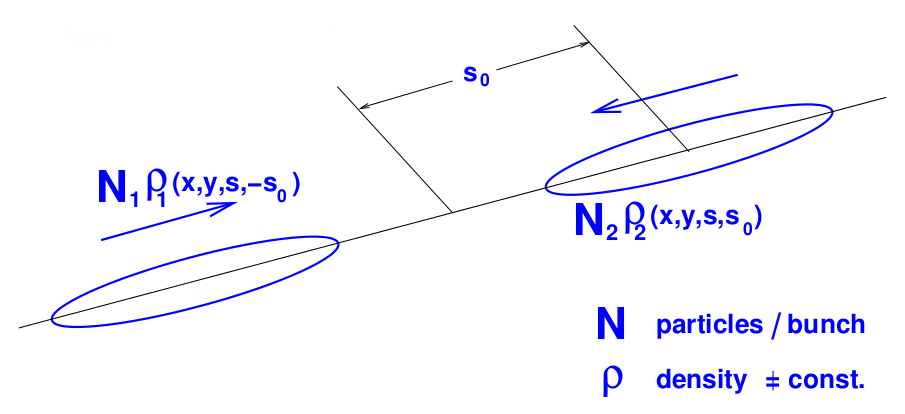
\includegraphics[width=0.75\linewidth]{../HourglassIntro/figs/simple_bunch_head_on.png}
\label{fig:xing_bunch}
\end{center}
\end{frame}

\begin{frame}{Introduction to $\beta^{*}$,  $\theta_{XZ}$ and $\theta_{YZ}$}
The simple normalized Gaussian beam profile for any single dimension, $x_i, i =
x, y, z$  may be
written, and normalized as follows:
\begin{equation}
\label{eq:simplegaussian}
\rho(x_{i}) = \frac{e^{ -\frac{(x_{i}-\mu)^2}{2\sigma_{x_i}^2}}}{\sigma_{x_i}\sqrt{2\pi}}
\end{equation}
If all profiles are of this form, then the densities are separable, and we may
perform the integration. However, higher order beam effects introduce
complications which will prevent us from separating the densities, as well as
performing the integration analytically.
\end{frame}

\begin{frame}{Introduction to $\beta^{*}$,  $\theta_{XZ}$ and $\theta_{YZ}$}
There are three transformations which we can perform on our profile, to generate
the most realistic overlap integral. Once we have a form that we are happy with,
we may integrate out the $x$ and $y$ degrees of freedom, leaving a distribution
in $z$ and $t$. This distribution is sampled randomly to create a simulated
z-vertex profile, which we can seed with experimentally extracted data, and tune
until sufficient convergence is achieved.
\end{frame}


\begin{frame}{Introduction to $\beta^{*}$,  $\theta_{XZ}$ and $\theta_{YZ}$}
The crossing angle may be applied in either the X-Z plane or Y-Z plane (or
both). Schematically:\\ 
\begin{columns}[T] % contents are top vertically aligned
\begin{column}[T]{5cm} % each column can also be its own environment
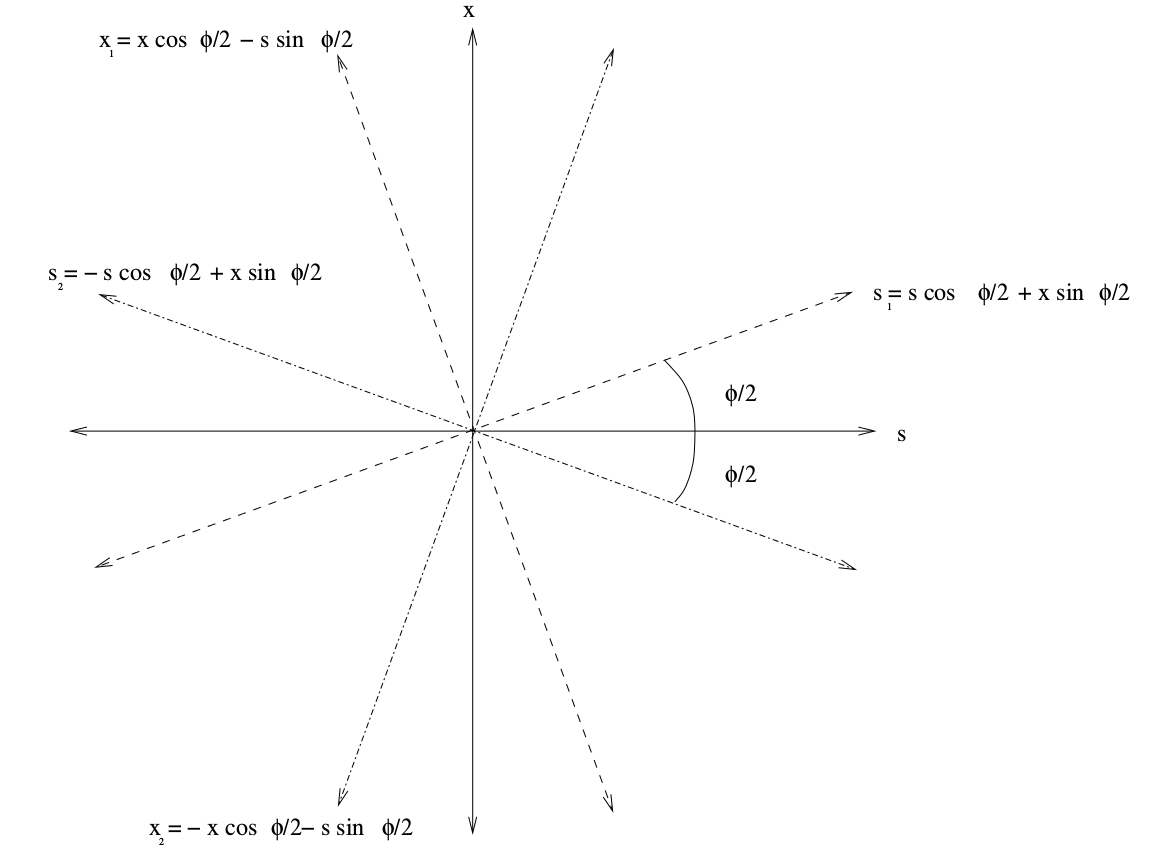
\includegraphics[width=\linewidth,height=\textheight,keepaspectratio]{../HourglassIntro/figs/bunch_rotation.png}
\end{column}
\begin{column}[T]{5cm} % alternative top-align that's better for graphics
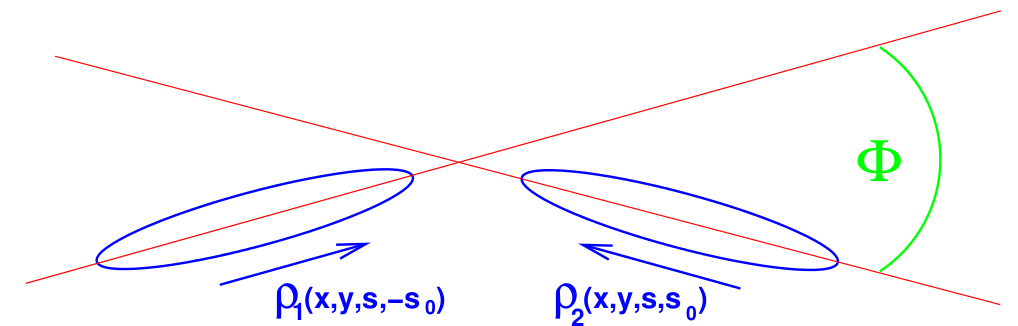
\includegraphics[width=\linewidth,height=\textheight,keepaspectratio]{../HourglassIntro/figs/xing_bunch.png}
\end{column}
\end{columns}
Left: rotation transformation, Right: bunches crossing at an angle, $\Phi$ relative to each-other.
\end{frame}

\begin{frame}{Introduction to $\beta^{*}$,  $\theta_{XZ}$ and $\theta_{YZ}$}
We transform our coordinate system, thus giving us shifted coordinates to
account for non-zero $\theta_{XZ}$ and $\theta_{YZ}$. Because crossing angles
are all small, $\nobreak(-0.2 rad < \theta < 0.2 rad)$, we can use the small angle
approximation.
\begin{gather}
\label{eq:transformations}
x_{blue}   \rightarrow x cos \frac{\phi}{2} - z sin \frac{\phi}{2} \\
z_{blue}   \rightarrow z cos \frac{\phi}{2} + x sin \frac{\phi}{2} \\
x_{yellow} \rightarrow x cos \frac{\phi}{2} + z sin \frac{\phi}{2} \\
z_{yellow} \rightarrow z cos \frac{\phi}{2} - z sin \frac{\phi}{2} \\
sin \frac {\phi}{2} \rightarrow \frac{\phi}{2} \\
cos \frac {\phi}{2} \rightarrow 1 + \frac{\phi^2}{4}
\end{gather}
\end{frame}

\begin{frame}{Introduction to $\beta^{*}$,  $\theta_{XZ}$ and $\theta_{YZ}$}
\begin{columns}[T] % contents are top vertically aligned
\begin{column}[T]{5cm} % each column can also be its own environment
To the left, we can see an example of a beta-function which effectively pinches
the transverse profiles of the beam down to a focused point at the center of the
interaction region. We must therefore transform the widths of our transverse
distributions like so:

\begin{equation}
\label{eq:beta_star_transform}
\sigma_{x_i} \rightarrow \sigma_{x_i} \sqrt{1+\left(\frac{z}{\beta^*}\right)^2 }
\end{equation}
\end{column}
\begin{column}[T]{5cm} % alternative top-align that's better for graphics
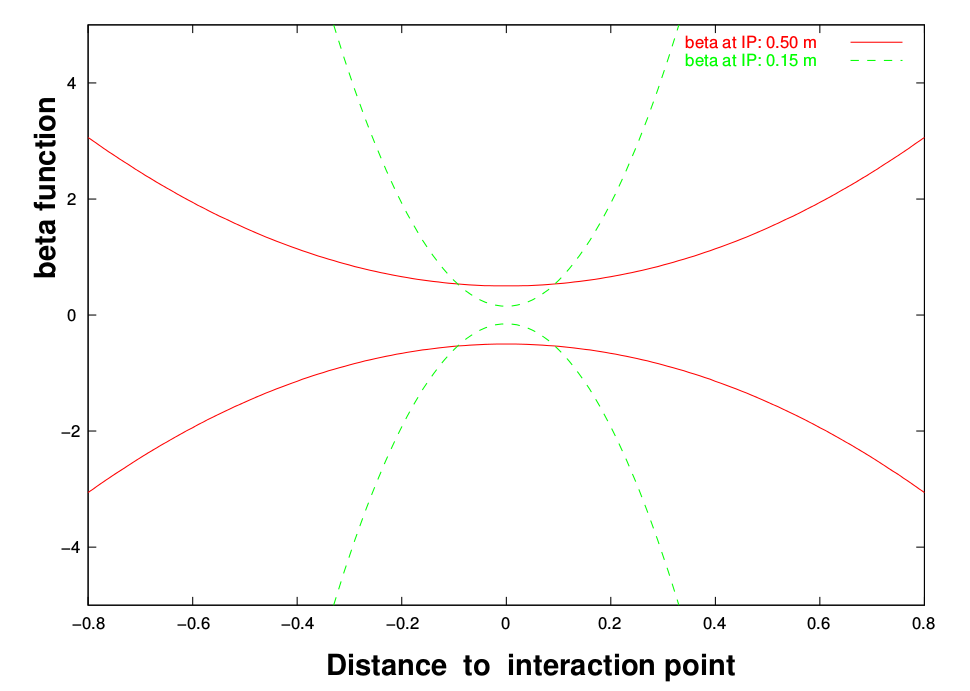
\includegraphics[width=\linewidth,height=\textheight,keepaspectratio]{../HourglassIntro/figs/beta_function.png}
\end{column}
\end{columns}
\end{frame}

\begin{frame}{Introduction to $\beta^{*}$,  $\theta_{XZ}$ and $\theta_{YZ}$}
The correction procedure:
\begin{itemize}
\item Begin with model for luminosity, make reasonable assumptions
\item Modify model to account for real effects
\item Numerically integrate to z-t distribution
\item Sample z-t distribution to obtain z-vertex profile
\item \textbf{Next:} Matching simulated distribution to data using statistically
	significant method (i.e., not "by eye" which has been done in past
	analyses"
\item \textbf{Next:} Correct luminosity by scaling simple model of luminosity of data to
	match simulated luminosity.
\end{itemize}
\end{frame}
